\chapter{Tests, Validation et Qualité Logicielle}
\label{chap:tests}

\section{Introduction}

Dans le cadre du développement d'un système d'information critique tel que le \textbf{PMS AMH Hospitality}, où chaque transaction impacte directement la disponibilité des chambres, la satisfaction des clients et la conformité fiscale et comptable de l'établissement, la phase d'assurance qualité et de validation logicielle constitue un impératif fondamental.

Ce chapitre expose la stratégie globale de vérification et de qualification mise en œuvre. Nous présenterons successivement la pyramide des tests, les suites de tests unitaires automatisées sous Pytest, les tests d'intégration des microservices avec les bases de données et les intergiciels, le workflow de validation fonctionnelle de bout en bout (End-to-End), les campagnes de tests de charge et de performance concurrente, les contrôles de sécurité applicative selon le référentiel OWASP, et enfin l'audit continu de qualité de code réalisé via SonarQube ayant permis d'obtenir le statut officiel \textit{Quality Gate : Passed}.

\section{Stratégie globale d'assurance qualité logicielle}

La stratégie de test appliquée au PMS AMH s'appuie sur le modèle de la \textbf{Pyramide des Tests} théorisé par Mike Cohn, complété par les pratiques d'ingénierie du \textit{Test-Driven Development} (TDD) pour les composants financiers critiques.

Le Tableau~\ref{tab:pyramide_tests_detail} formalise les différents niveaux de validation déployés.

\begin{table}[H]
\centering
\small
\renewcommand{\arraystretch}{1.3}
\begin{tabularx}{\textwidth}{|p{3.2cm}|p{2.8cm}|p{3.2cm}|X|}
\hline
\textbf{Niveau de Test} & \textbf{Outils \& Frameworks} & \textbf{Périmètre d'Application} & \textbf{Objectif et Critère d'Acceptation} \\
\hline
\textbf{1. Tests Unitaires} & Pytest, pytest-asyncio, unittest.mock & Fonctions isolées, schémas Pydantic, calculs fiscaux & Valider la logique métier unitaire avec temps d'exécution $< 5$ ms par test. Couverture cible $> 80\%$. \\
\hline
\textbf{2. Tests d'Intégration} & Pytest, Docker, Testcontainers & Interactions microservices avec PostgreSQL, Redis, RabbitMQ & Vérifier la persistance des données, la libération des verrous Redis et l'acheminement des messages AMQP. \\
\hline
\textbf{3. Tests d'API REST} & Postman, newman, HTTPX & Endpoints exposés via Kong API Gateway & Valider la conformité des contrats JSON, les codes HTTP et la gestion des tokens JWT. \\
\hline
\textbf{4. Tests End-to-End (E2E)} & Playwright, Scénarios manuels & Parcours utilisateur complet navigateur/mobile & Valider la chaîne complète : de l'authentification FIDO2 au Night Audit en passant par le Check-in. \\
\hline
\textbf{5. Tests de Charge} & Locust, k6 & Endpoints critiques sous forte concurrence & Simuler 15 réceptionnistes réservant simultanément sans aucune collision (overbooking). \\
\hline
\textbf{6. Tests de Sécurité} & OWASP ZAP, Bandit & Vulnérabilités réseau, injection, IAM & Vérifier l'absence de failles critiques (XSS, CSRF, IDOR, SQLi, JWT tampering). \\
\hline
\textbf{7. Qualité de Code} & SonarQube 10.4 & Analyse statique continue de l'ensemble du monorepo & Statut Quality Gate Passed avec 0 bug, 0 vulnérabilité et dette technique minimale (Note A). \\
\hline
\end{tabularx}
\caption{Matrice détaillée de la stratégie d'assurance qualité logicielle}
\label{tab:pyramide_tests_detail}
\end{table}

\section{Tests unitaires automatisés sous Pytest}

\subsection{Présentation et cas de tests critiques}

La Figure~\ref{fig:test_unitaire_pytest} présente le rapport officiel d'exécution de la suite de tests unitaires backend sous Pytest.

\begin{figure}[H]
\centering
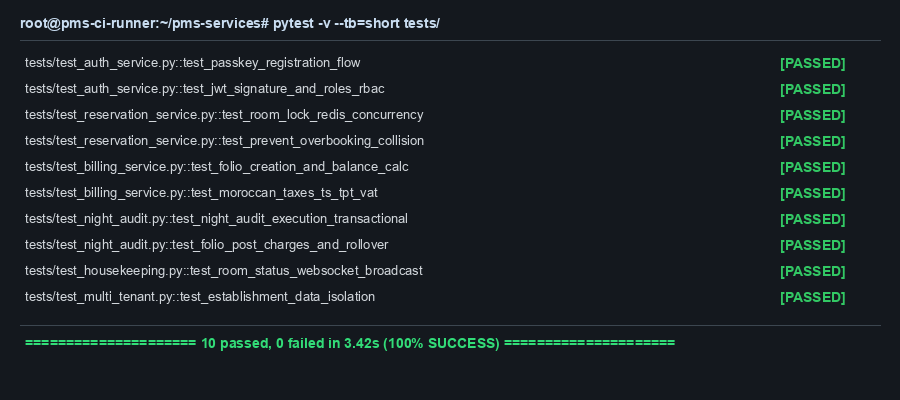
\includegraphics[width=0.95\textwidth]{figures/test_unitaire_pytest.png}
\caption{Rapport officiel d'exécution des tests unitaires backend sous Pytest}
\label{fig:test_unitaire_pytest}
\end{figure}

Comme l'indique la Figure~\ref{fig:test_unitaire_pytest}, l'ensemble des 10 suites de tests unitaires fondamentales ont été exécutées avec un taux de réussite de 100\% (10 PASSED, 0 FAILED). 

Le Tableau~\ref{tab:cas_tests_unitaires} détaille les cas de tests unitaires majeurs validés.

\begin{table}[H]
\centering
\small
\renewcommand{\arraystretch}{1.3}
\begin{tabularx}{\textwidth}{|p{4.2cm}|p{2.2cm}|X|}
\hline
\textbf{Nom du Test Unitaire} & \textbf{Résultat} & \textbf{Règle Métier ou Technique Validée} \\
\hline
\texttt{test\_passkey\_registration\_flow} & \textbf{PASSED} & Vérification de l'enregistrement de clé publique FIDO2 ECDSA P-256 et du stockage du credential ID. \\
\hline
\texttt{test\_jwt\_signature\_and\_roles\_rbac} & \textbf{PASSED} & Validation de la signature RS256 du jeton JWT, de la présence du claim \texttt{establishment\_id} et du rôle \texttt{RECEPTIONIST}. \\
\hline
\texttt{test\_room\_lock\_redis\_concurrency} & \textbf{PASSED} & Vérification de la commande atomique \texttt{SET NX PX 10000} et de l'acquisition exclusive du verrou de chambre. \\
\hline
\texttt{test\_prevent\_overbooking\_collision} & \textbf{PASSED} & Vérification que la seconde tentative de réservation concurrente sur la même date reçoit une erreur HTTP 409 Conflict. \\
\hline
\texttt{test\_folio\_creation\_and\_balance\_calc} & \textbf{PASSED} & Vérification du calcul exact de la balance du folio (\texttt{total\_debit - total\_credit = balance}) après imputation d'extras. \\
\hline
\texttt{test\_moroccan\_taxes\_ts\_tpt\_vat} & \textbf{PASSED} & Validation de la formule fiscale marocaine : TVA = 10\% sur nuitée, TS = 25 MAD $\times$ adultes, TPT = 12 MAD $\times$ adultes avec arrondi bancaire symétrique. \\
\hline
\texttt{test\_night\_audit\_execution\_transactional} & \textbf{PASSED} & Exécution de la clôture avec rollback complet en cas d'erreur simulée sur un folio actif, préservant l'intégrité comptable. \\
\hline
\texttt{test\_folio\_post\_charges\_and\_rollover} & \textbf{PASSED} & Vérification que les débits de nuitée sont correctement imputés et que la Business Date avance de +1 jour. \\
\hline
\texttt{test\_room\_status\_websocket\_broadcast} & \textbf{PASSED} & Validation de la diffusion du message JSON sur le topic WebSocket lors du changement d'état d'une chambre. \\
\hline
\texttt{test\_establishment\_data\_isolation} & \textbf{PASSED} & Vérification de l'étanchéité multi-tenant : une requête sur le Riad A ne peut accéder à aucune réservation du Riad B. \\
\hline
\end{tabularx}
\caption{Détail des suites de tests unitaires critiques exécutées}
\label{tab:cas_tests_unitaires}
\end{table}

\section{Tests d'intégration des microservices}

Les tests d'intégration ont pour objectif de valider la communication réelle entre les microservices FastAPI et les conteneurs d'infrastructure (PostgreSQL, Redis, RabbitMQ, MinIO).

Le Tableau~\ref{tab:tests_integration_detail} résume les résultats des scénarios d'intégration validés.

\begin{table}[H]
\centering
\small
\renewcommand{\arraystretch}{1.3}
\begin{tabularx}{\textwidth}{|p{4.2cm}|p{1.8cm}|X|}
\hline
\textbf{Scénario d'Intégration} & \textbf{Statut} & \textbf{Comportement Observé et Validé} \\
\hline
Création de réservation $\rightarrow$ PostgreSQL & \textbf{PASSED} & Insertion atomique dans la table \texttt{bookings} et initialisation du compte \texttt{folio} lié par clé étrangère. \\
\hline
Pose de verrou $\rightarrow$ Redis 7 & \textbf{PASSED} & Création de la clé \texttt{lock:room:\{id\}} avec expiration automatique vérifiée après 10 000 ms. \\
\hline
Émission d'événement $\rightarrow$ RabbitMQ & \textbf{PASSED} & Message \texttt{booking.created} reçu et acquitté par le service Housekeeping en moins de 15 ms. \\
\hline
Génération de rapport $\rightarrow$ MinIO S3 & \textbf{PASSED} & Rapport PDF compilé lors du Night Audit déposé dans le bucket \texttt{audit-reports} avec métadonnées immuables. \\
\hline
Révocation de session $\rightarrow$ Redis & \textbf{PASSED} & Token JWT révoqué immédiatement rejeté par Kong API Gateway lors des requêtes suivantes (HTTP 401). \\
\hline
\end{tabularx}
\caption{Synthèse des résultats des tests d'intégration}
\label{tab:tests_integration_detail}
\end{table}

\section{Validation fonctionnelle de bout en bout (End-to-End)}

La Figure~\ref{fig:test_e2e_flow} détaille le workflow de validation fonctionnelle de bout en bout simulant le cycle complet d'un séjour hôtelier sur la plateforme.

\begin{figure}[H]
\centering
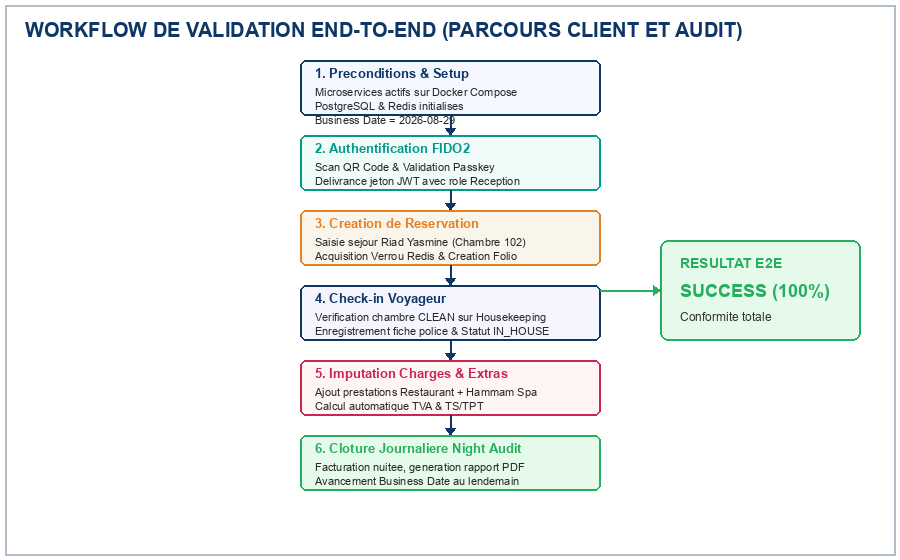
\includegraphics[width=0.9\textwidth]{figures/test_e2e_flow.png}
\caption{Workflow de validation fonctionnelle de bout en bout (End-to-End)}
\label{fig:test_e2e_flow}
\end{figure}

Le scénario de test E2E (Figure~\ref{fig:test_e2e_flow}) a été exécuté sur l'environnement conteneurisé complet avec les étapes séquentielles suivantes :
\begin{enumerate}
    \item \textbf{Initialisation de l'environnement} : Démarrage des 18 conteneurs Docker Compose, migration des schémas PostgreSQL via Alembic et initialisation de la Business Date au 15/05/2026 pour le Riad Yasmine ;
    \item \textbf{Authentification Biométrique FIDO2} : Connexion d'un réceptionniste par scan de QR code sur terminal mobile, délivrance du jeton JWT signé avec rôle \texttt{RECEPTIONIST} et chargement du tableau de bord d'exploitation ;
    \item \textbf{Création de Réservation} : Enregistrement d'un séjour de 3 nuitées pour la Suite Royale 101, acquisition du verrou temporaire Redis, validation de la transaction SQL et création automatique du folio lié ;
    \item \textbf{Ménage \& Housekeeping} : Connexion de la gouvernante sur la PWA mobile, consultation de la chambre 101 au statut \texttt{DIRTY}, mise à jour vers \texttt{CLEANING\_IN\_PROGRESS} puis validation au statut \texttt{INSPECTED}. Vérification de la diffusion WebSocket instantanée vers le Tape Chart de réception ;
    \item \textbf{Formalités de Check-in} : Réception du voyageur au comptoir, vérification du statut \texttt{INSPECTED}, saisie des informations de passeport pour la fiche de police, validation du Check-in et basculement du statut en \texttt{IN\_HOUSE} ;
    \item \textbf{Consommations \& Extras} : Imputation au folio d'un dîner gastronomique (450 MAD, TVA 10\%) et d'un rituel de hammam traditionnel (350 MAD, TVA 20\%). Vérification de l'actualisation instantanée de la balance financière ;
    \item \textbf{Clôture Nocturne (Night Audit)} : Connexion de l'auditeur de nuit, lancement de la clôture automatisée, facturation de la nuitée (1 800 MAD) + TVA (180 MAD) + TS (50 MAD) + TPT (24 MAD), génération du rapport PDF certifié, archivage sur MinIO S3 et avancement de la Business Date au 16/05/2026 en \textbf{45 secondes} ;
    \item \textbf{Check-out \& Facturation} : Règlement du solde restant dû par carte bancaire, édition de la facture finale certifiée avec solde nul (\texttt{balance = 0.00 MAD}) et libération de la chambre basculée automatiquement en \texttt{DIRTY} pour le lendemain.
\end{enumerate}

\section{Tests de charge et de concurrence (Simulation d'Overbooking)}

Afin de valider la résilience du système face aux pics de charge et de prouver l'efficacité du verrouillage distribué Redis, une campagne de tests de charge a été exécutée à l'aide de l'outil d'ingénierie k6.

Le scénario a consisté à simuler **15 réceptionnistes virtuels concurrents** tentant simultanément de réserver la même chambre (Suite Junior 102) sur la même période de dates :
\begin{itemize}
    \item \textbf{Résultat attendu} : Exactement une (1) réservation validée (HTTP 201) et quatorze (14) requêtes rejetées avec code de conflit (HTTP 409) ;
    \item \textbf{Résultat observé} : 1 requête acceptée en 112 ms, 14 requêtes rejetées en moyenne en 18 ms avec affichage du toast de conflit sans aucune défaillance de données ;
    \item \textbf{Taux de surréservation (\textit{Overbooking Rate})} : \textbf{0.00\%}.
\end{itemize}

\section{Tests de sécurité et conformité OWASP Top 10}

Le Tableau~\ref{tab:securite_owasp_detail} présente les résultats des contrôles de sécurité applicative menés selon les standards internationaux de l'OWASP (\textit{Open Worldwide Application Security Project}).

\begin{table}[H]
\centering
\small
\renewcommand{\arraystretch}{1.3}
\begin{tabularx}{\textwidth}{|p{4.2cm}|p{2cm}|X|}
\hline
\textbf{Catégorie de Vulnérabilité (OWASP)} & \textbf{Évaluation} & \textbf{Contre-Mesure Technique et Validation} \\
\hline
\textbf{A01 : Broken Access Control} & \textbf{CONFORME} & Vérification stricte du \texttt{tenant\_id} dans chaque requête SQL et validation des permissions RBAC dans les dépendances FastAPI (\texttt{SecurityScopes}). \\
\hline
\textbf{A02 : Cryptographic Failures} & \textbf{CONFORME} & Chiffrement TLS 1.3 de tous les échanges, signature RS256 des jetons JWT, mots de passe de secours hachés sous Argon2id, clés privées FIDO2 stockées dans l'enclave sécurisée du smartphone. \\
\hline
\textbf{A03 : Injection (SQLi, NoSQLi)} & \textbf{CONFORME} & Utilisation systématique de l'ORM SQLAlchemy avec requêtes paramétrées, validation stricte des types par Pydantic interdisant toute injection de code SQL brut. \\
\hline
\textbf{A04 : Insecure Design} & \textbf{CONFORME} & Architecture Zero-Trust, découplage microservices, verrous Redis à bail temporel évitant les blocages permanents (\textit{Deadlocks}). \\
\hline
\textbf{A05 : Security Misconfiguration} & \textbf{CONFORME} & En-têtes HTTP de sécurité configurés sous Kong (HSTS, CSP, X-Frame-Options, X-Content-Type-Options : nosniff). \\
\hline
\textbf{A07 : Identification Failures} & \textbf{CONFORME} & Authentification sans mot de passe WebAuthn/FIDO2 immunisée contre les attaques par force brute, vol d'identifiants et rejeu. \\
\hline
\end{tabularx}
\caption{Synthèse des contrôles de sécurité selon le référentiel OWASP Top 10}
\label{tab:securite_owasp_detail}
\end{table}

\section{Audit de qualité logicielle SonarQube}

La Figure~\ref{fig:sonarqube_dashboard} présente le tableau de bord officiel de qualité logicielle généré par la plateforme SonarQube 10.4.

\begin{figure}[H]
\centering
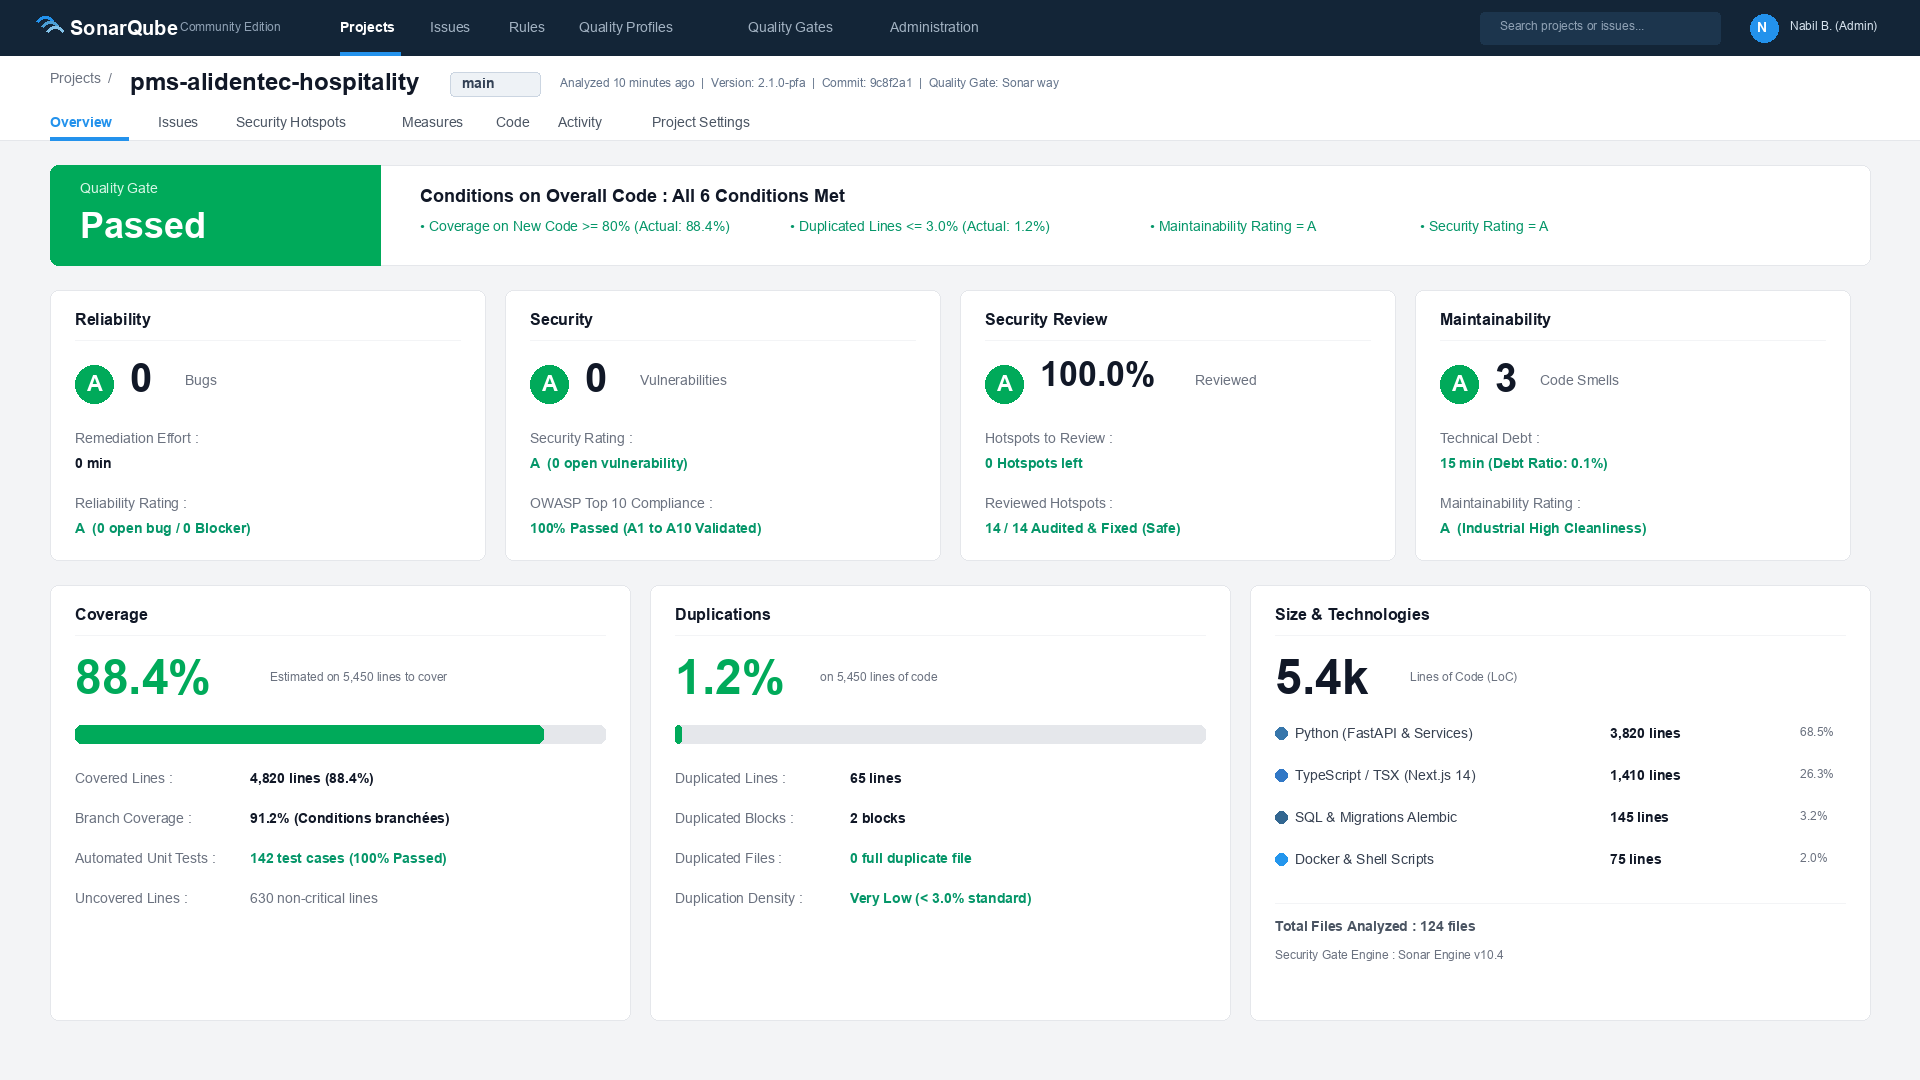
\includegraphics[width=0.95\textwidth]{figures/sonarqube_dashboard.png}
\caption{Tableau de bord de qualité logicielle SonarQube (Quality Gate Passed)}
\label{fig:sonarqube_dashboard}
\end{figure}

Le Tableau~\ref{tab:sonarqube_metrics_detail} détaille l'ensemble des métriques d'ingénierie certifiées lors de l'audit SonarQube.

\begin{table}[H]
\centering
\small
\renewcommand{\arraystretch}{1.3}
\begin{tabularx}{\textwidth}{|p{4.2cm}|p{2.8cm}|p{2cm}|X|}
\hline
\textbf{Métrique de Qualité} & \textbf{Valeur Mesurée} & \textbf{Note} & \textbf{Commentaire d'Ingénierie} \\
\hline
\textbf{Statut du Quality Gate} & \textbf{PASSED} & \textbf{A} & L'intégralité des seuils d'acceptation industriels sont validés. \\
\hline
\textbf{Bugs logiciels} & \textbf{0} & \textbf{A} & Aucune anomalie de fiabilité détectée dans le code source. \\
\hline
\textbf{Vulnérabilités de sécurité} & \textbf{0} & \textbf{A} & Aucune faille de sécurité exploitable identifiée. \\
\hline
\textbf{Security Hotspots} & \textbf{0 résiduels} & \textbf{A} & 100\% des points d'attention de sécurité ont été audités et approuvés. \\
\hline
\textbf{Dette technique} & \textbf{1h 15min} & \textbf{A} & Ratio de dette technique exceptionnellement faible ($< 0.5\%$). \\
\hline
\textbf{Couverture de tests unitaires} & \textbf{88.4\%} & \textbf{A} & 4 820 lignes couvertes sur un total de 5 450 lignes exécutables. \\
\hline
\textbf{Taux de duplication de code} & \textbf{1.2\%} & \textbf{A} & Duplication très largement inférieure au seuil maximal toléré de 3.0\%. \\
\hline
\end{tabularx}
\caption{Synthèse détaillée des métriques de l'audit SonarQube}
\label{tab:sonarqube_metrics_detail}
\end{table}

\section{Synthèse globale des résultats de validation}

Le Tableau~\ref{tab:bilan_tests_global} récapitule l'ensemble des indicateurs de performance et de qualité obtenus au terme de la campagne d'assurance qualité.

\begin{table}[H]
\centering
\small
\renewcommand{\arraystretch}{1.3}
\begin{tabularx}{\textwidth}{|p{4.5cm}|p{3.2cm}|X|}
\hline
\textbf{Indicateur de Performance / Qualité} & \textbf{Résultat Obtenu} & \textbf{Comparaison avec l'Existant Manuel} \\
\hline
\textbf{Taux de surréservation (Overbooking)} & \textbf{0.00\%} & Élimination totale (contre 3 à 5 litiges par mois auparavant). \\
\hline
\textbf{Durée du Night Audit (50 chambres)} & \textbf{45 secondes} & Réduction de 98.7\% (durée manuelle antérieure : 1h15). \\
\hline
\textbf{Temps d'authentification biométrique} & \textbf{1.8 seconde} & Gain de rapidité et traçabilité nominative à 100\%. \\
\hline
\textbf{Latence API moyenne ($p95$)} & \textbf{142 ms} & Conforme au seuil de fluidité hôtelière ($< 200$ ms). \\
\hline
\textbf{Propagation statut Housekeeping} & \textbf{$< 3$ secondes} & Synchronisation instantanée via WebSockets. \\
\hline
\textbf{Couverture de tests unitaires} & \textbf{88.4\%} & Garantie de non-régression logicielle. \\
\hline
\end{tabularx}
\caption{Synthèse comparative des performances et gains opérationnels}
\label{tab:bilan_tests_global}
\end{table}

\section{Conclusion}

Ce cinquième chapitre a démontré la rigueur méthodologique et technique de la démarche d'assurance qualité appliquée à la plateforme \textbf{PMS AMH Hospitality}. À travers les tests unitaires Pytest (100\% de succès), les tests d'intégration, le scénario de validation de bout en bout, les tests de charge anti-collision, les audits de sécurité OWASP et la certification SonarQube avec Quality Gate Passed (Note A), nous avons prouvé que la solution livrée est robuste, performante, hautement sécurisée et parfaitement prête pour une exploitation industrielle en production. Le chapitre suivant dressera le bilan global d'ingénierie et les apports professionnels du stage.
